\documentclass[3p,a4paper,11pt,review]{elsarticle}

\usepackage{lineno}
\usepackage{hyperref}
\usepackage{latexsym}
\usepackage{color}
\usepackage[table]{xcolor}
\usepackage{mathrsfs}
\usepackage{amssymb,amstext,amsfonts,amsmath,amsthm}
\usepackage{bm}
\usepackage{subcaption}
\usepackage[utf8]{inputenc} 
\usepackage[english]{babel}
\usepackage{hyphenat}
\usepackage{calc}
\usepackage{graphicx,import}

\usepackage{soul}

\usepackage{caption}
\usepackage{subcaption}

\usepackage{arydshln}
\usepackage{natbib}
\usepackage[misc,geometry]{ifsym} 
\usepackage{empheq}
\usepackage{longtable}
\usepackage{comment}

\bibliographystyle{plain}\biboptions{authoryear}


\usepackage{lineno}
\newcommand*\patchAmsMathEnvironmentForLineno[1]{%
	\expandafter\let\csname old#1\expandafter\endcsname\csname #1\endcsname
	\expandafter\let\csname oldend#1\expandafter\endcsname\csname end#1\endcsname
	\renewenvironment{#1}%
	{\linenomath\csname old#1\endcsname}%
	{\csname oldend#1\endcsname\endlinenomath}}%
\newcommand*\patchBothAmsMathEnvironmentsForLineno[1]{%
	\patchAmsMathEnvironmentForLineno{#1}%
	\patchAmsMathEnvironmentForLineno{#1*}}%
\AtBeginDocument{%
	\patchBothAmsMathEnvironmentsForLineno{equation}%
	\patchBothAmsMathEnvironmentsForLineno{align}%
	\patchBothAmsMathEnvironmentsForLineno{flalign}%
	\patchBothAmsMathEnvironmentsForLineno{alignat}%
	\patchBothAmsMathEnvironmentsForLineno{gather}%
	\patchBothAmsMathEnvironmentsForLineno{multline}%
}

\usepackage[]{algorithm2e}

\hyphenation{ONSAS}

\usepackage{tikz}
\usetikzlibrary{shapes,arrows}

\usepackage{relsize}

\definecolor{darkcandyapplered}{rgb}{0.64, 0.0, 0.0}
\definecolor{darkred}{rgb}{0.55, 0.0, 0.0}


\usepackage{bbm}



\usepackage{enumitem,amssymb}
\newlist{todolist}{itemize}{2}
\setlist[todolist]{label=$\square$}
%
\usepackage{pifont}
%
\newcommand{\failed}{%
	\rlap{\raisebox{0.3ex}{\hspace{0.4ex}\scriptsize \ding{56}}}$\square$%
}
%
\newcommand{\done}{%
	\rlap{\raisebox{0.3ex}{\hspace{0.4ex}\tiny \ding{52}}}$\square$%
}

\newcommand{\miparra}[1]{\vspace{5mm} \textbf{#1}\\}

\journal{?}

\begin{document}
	
	
	\begin{frontmatter}
		
		\title{A Consistent Co-rotational Formulation for Quasi-Steady Aerodynamic Nonlinear Analysis of Frame Structures}
		
		\author[1]{Mauricio C. Vanzulli}
		\author[2]{Jorge M. Pérez Zerpa}
		
		\address[1]{Instituto de Ingeniería Mecánica y Producción Industrial, Facultad de Ingeniería, Universidad de la República, Montevideo, Uruguay}
		
		% Corresponding author
		\address[2]{Instituto de Estructuras y Transporte, Facultad de Ingeniería, Universidad de la República, Montevideo, Uruguay}  
		
	\end{frontmatter}


\section{Numerical results}



\newcommand{\CantileverBladeL}{10}
\newcommand{\CantileverBladedch}{1}
\newcommand{\CantileverBladeEeq}{14}
\newcommand{\CantileverBladeGeq}{  5.6}
\newcommand{\CantileverBladerho}{1850}
\newcommand{\CantileverBladevm}{30}
\newcommand{\CantileverBladetolF}{5}
\newcommand{\CantileverBladetolU}{1}
\newcommand{\CantileverBladedeltaT}{1}
\newcommand{\CantileverBladefinalTime}{30}
\newcommand{\CantileverBladenumElem}{10}
\newcommand{\CantileverBladealphaEnd}{   40}
\newcommand{\CantileverBladetorsionalMomentRatio}{-67745}
\newcommand{\CantileverBladetorsionalMomentFOne}{ 0.03}
\newcommand{\CantileverBladetorsionalMomentFTwo}{-1819}


\subsection{Example 3}


\subsubsection{Parameters}
The parameters of this example are:

\begin{itemize}
	\item $d_c= \CantileverBladedch$ 
	\item $L = \CantileverBladeL$
	\item $E_{eq} = \CantileverBladeEeq$ GPa
	\item $G_{eq} = \CantileverBladeGeq$ GPa
	\item $v_{m} = \CantileverBladevm$ m/s
	\item $tol_r = \CantileverBladetolF\times 10^{-7}$
	\item $tol_u = \CantileverBladetolU0^{-15}$.
	\item $\alpha = \CantileverBladealphaEnd^{\circ}$
\end{itemize}


\subsubsection{Numerical results}


The torsional moment provided by geometric nonlinearities in F1 is $\CantileverBladetorsionalMomentFOne$ N.m while using F2 is $\CantileverBladetorsionalMomentFTwo$ N.m


\begin{figure}[htb]
	\begin{subfigure}{.5\textwidth}
		\centering
		\resizebox{.9\textwidth}{!}{% Title: Figure 5
% Creator: GL2PS 1.4.2, (C) 1999-2020 C. Geuzaine
% For: Octave
% CreationDate: Mon Jan 23 19:18:48 2023
\setlength{\unitlength}{1pt}
\begin{picture}(0,0)
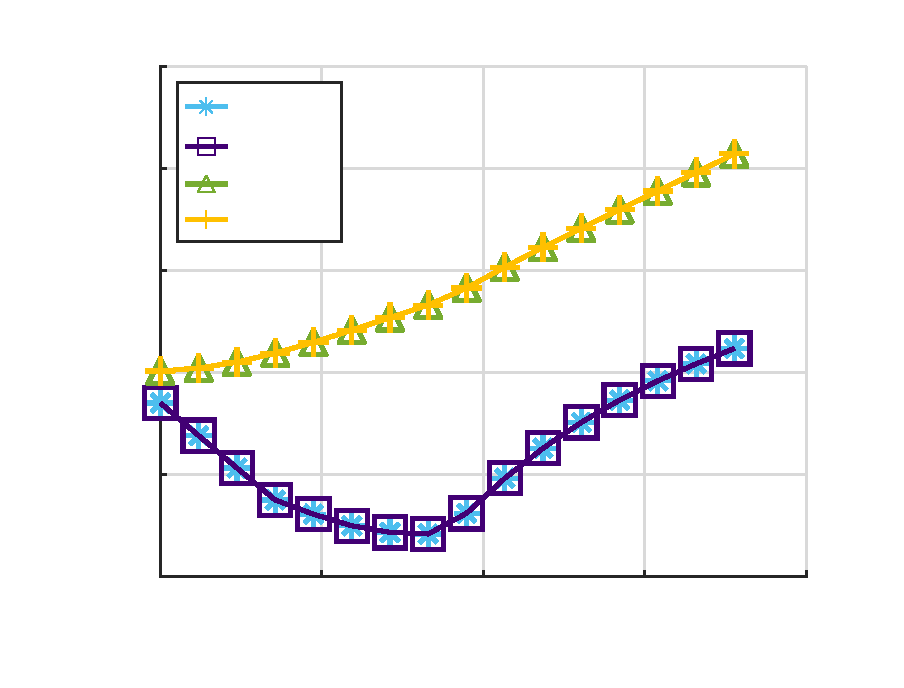
\includegraphics[scale=1]{BladeCantMomentsYZStatic-inc}
\end{picture}%
\begin{picture}(418,314)(0,0)
\fontsize{18}{0}\selectfont\put(85.9984,42.9568){\makebox(0,0)[t]{\textcolor[rgb]{0.15,0.15,0.15}{{$0$}}}}
\fontsize{18}{0}\selectfont\put(159.235,42.9568){\makebox(0,0)[t]{\textcolor[rgb]{0.15,0.15,0.15}{{$\pi/16$}}}}
\fontsize{18}{0}\selectfont\put(232.472,42.9568){\makebox(0,0)[t]{\textcolor[rgb]{0.15,0.15,0.15}{{$\pi/8$}}}}
\fontsize{18}{0}\selectfont\put(305.709,42.9568){\makebox(0,0)[t]{\textcolor[rgb]{0.15,0.15,0.15}{{$3\pi/16$}}}}
\fontsize{18}{0}\selectfont\put(378.946,42.9568){\makebox(0,0)[t]{\textcolor[rgb]{0.15,0.15,0.15}{{$\pi/4$}}}}
\fontsize{18}{0}\selectfont\put(77,56.4563){\makebox(0,0)[r]{\textcolor[rgb]{0.15,0.15,0.15}{{-10000}}}}
\fontsize{18}{0}\selectfont\put(77,95.4547){\makebox(0,0)[r]{\textcolor[rgb]{0.15,0.15,0.15}{{0}}}}
\fontsize{18}{0}\selectfont\put(77,134.453){\makebox(0,0)[r]{\textcolor[rgb]{0.15,0.15,0.15}{{10000}}}}
\fontsize{18}{0}\selectfont\put(77,173.451){\makebox(0,0)[r]{\textcolor[rgb]{0.15,0.15,0.15}{{20000}}}}
\fontsize{18}{0}\selectfont\put(77,212.45){\makebox(0,0)[r]{\textcolor[rgb]{0.15,0.15,0.15}{{30000}}}}
\fontsize{18}{0}\selectfont\put(77,251.448){\makebox(0,0)[r]{\textcolor[rgb]{0.15,0.15,0.15}{{40000}}}}
\fontsize{18}{0}\selectfont\put(77,290.447){\makebox(0,0)[r]{\textcolor[rgb]{0.15,0.15,0.15}{{50000}}}}
\fontsize{18}{0}\selectfont\put(232.472,18.9568){\makebox(0,0)[t]{\textcolor[rgb]{0.15,0.15,0.15}{{$\alpha$ [rad]}}}}
\fontsize{18}{0}\selectfont\put(21,173.451){\rotatebox{90}{\makebox(0,0)[b]{\textcolor[rgb]{0.15,0.15,0.15}{{$M_z$, $M_y$ node O [N.m]}}}}}
\fontsize{16}{0}\selectfont\put(121.983,268.952){\makebox(0,0)[l]{\textcolor[rgb]{0,0,0}{{F1 $M_y$}}}}
\fontsize{16}{0}\selectfont\put(121.983,245.954){\makebox(0,0)[l]{\textcolor[rgb]{0,0,0}{{F2 $M_y$}}}}
\fontsize{16}{0}\selectfont\put(121.983,224.455){\makebox(0,0)[l]{\textcolor[rgb]{0,0,0}{{F1 $M_z$}}}}
\fontsize{16}{0}\selectfont\put(121.983,204.457){\makebox(0,0)[l]{\textcolor[rgb]{0,0,0}{{F2 $M_z$}}}}
\end{picture}
}		
		\caption{$M_y, M_z(\alpha)$.}
		\label{fig:BladeCantMYMZStatic}
	\end{subfigure}
	\begin{subfigure}{0.5\textwidth}
		\centering
		\resizebox{.9\textwidth}{!}{% Title: Figure 3
% Creator: GL2PS 1.4.2, (C) 1999-2020 C. Geuzaine
% For: Octave
% CreationDate: Sat Jan 21 18:26:39 2023
\setlength{\unitlength}{1pt}
\begin{picture}(0,0)
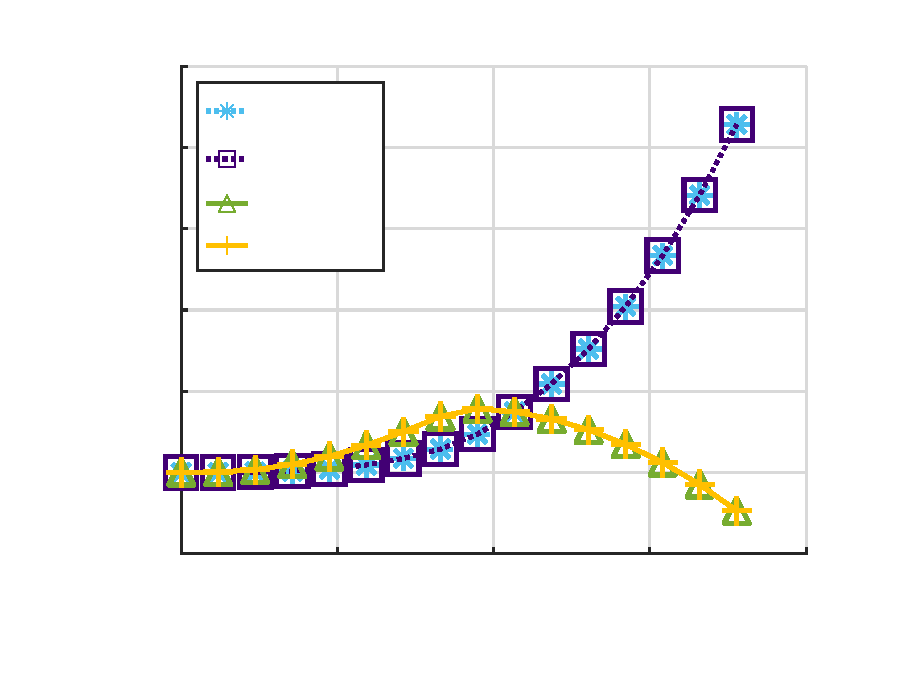
\includegraphics[scale=1]{BladeCantForcesStatic-inc}
\end{picture}%
\begin{picture}(418,314)(0,0)
\fontsize{18}{0}\selectfont\put(78.998,42.9569){\makebox(0,0)[t]{\textcolor[rgb]{0.15,0.15,0.15}{{$0$}}}}
\fontsize{18}{0}\selectfont\put(153.985,42.9569){\makebox(0,0)[t]{\textcolor[rgb]{0.15,0.15,0.15}{{$\pi/16$}}}}
\fontsize{18}{0}\selectfont\put(228.972,42.9569){\makebox(0,0)[t]{\textcolor[rgb]{0.15,0.15,0.15}{{$\pi/8$}}}}
\fontsize{18}{0}\selectfont\put(303.959,42.9569){\makebox(0,0)[t]{\textcolor[rgb]{0.15,0.15,0.15}{{$3\pi/16$}}}}
\fontsize{18}{0}\selectfont\put(378.946,42.9569){\makebox(0,0)[t]{\textcolor[rgb]{0.15,0.15,0.15}{{$\pi/4$}}}}
\fontsize{18}{0}\selectfont\put(69.9996,56.4563){\makebox(0,0)[r]{\textcolor[rgb]{0.15,0.15,0.15}{{-2000}}}}
\fontsize{18}{0}\selectfont\put(69.9996,95.4547){\makebox(0,0)[r]{\textcolor[rgb]{0.15,0.15,0.15}{{0}}}}
\fontsize{18}{0}\selectfont\put(69.9996,134.453){\makebox(0,0)[r]{\textcolor[rgb]{0.15,0.15,0.15}{{2000}}}}
\fontsize{18}{0}\selectfont\put(69.9996,173.452){\makebox(0,0)[r]{\textcolor[rgb]{0.15,0.15,0.15}{{4000}}}}
\fontsize{18}{0}\selectfont\put(69.9996,212.45){\makebox(0,0)[r]{\textcolor[rgb]{0.15,0.15,0.15}{{6000}}}}
\fontsize{18}{0}\selectfont\put(69.9996,251.448){\makebox(0,0)[r]{\textcolor[rgb]{0.15,0.15,0.15}{{8000}}}}
\fontsize{18}{0}\selectfont\put(69.9996,290.447){\makebox(0,0)[r]{\textcolor[rgb]{0.15,0.15,0.15}{{10000}}}}
\fontsize{18}{0}\selectfont\put(228.972,18.9569){\makebox(0,0)[t]{\textcolor[rgb]{0.15,0.15,0.15}{{$\alpha$ [rad]}}}}
\fontsize{18}{0}\selectfont\put(20.9996,173.452){\rotatebox{90}{\makebox(0,0)[b]{\textcolor[rgb]{0.15,0.15,0.15}{{$F_y$, $F_z$ node O [N]}}}}}
\fontsize{16}{0}\selectfont\put(114.982,268.952){\makebox(0,0)[l]{\textcolor[rgb]{0,0,0}{{F1 $F_y$}}}}
\fontsize{16}{0}\selectfont\put(114.982,245.954){\makebox(0,0)[l]{\textcolor[rgb]{0,0,0}{{F2 $F_y$}}}}
\fontsize{16}{0}\selectfont\put(114.982,224.455){\makebox(0,0)[l]{\textcolor[rgb]{0,0,0}{{F1 $F_z$}}}}
\fontsize{16}{0}\selectfont\put(114.982,204.457){\makebox(0,0)[l]{\textcolor[rgb]{0,0,0}{{F2 $F_z$}}}}
\end{picture}
}		
		\caption{$F_y$, $F_z$ $(\alpha)$.}
		\label{fig:BladeCantForcesStatic}
	\end{subfigure}
	\caption{Example 3: Reaction bending moments $M_y(\alpha)$, $M_z(\alpha)$ and resultant shear forces $F_y(\alpha)$ and $F_z(\alpha)$ at node O.}
	\label{fig:BladeCantStaticBending}
\end{figure}

\begin{figure}[htb]
	\centering
	\resizebox{.45\textwidth}{!}{% Title: Figure 4
% Creator: GL2PS 1.4.2, (C) 1999-2020 C. Geuzaine
% For: Octave
% CreationDate: Sat Jan 21 18:26:42 2023
\setlength{\unitlength}{1pt}
\begin{picture}(0,0)
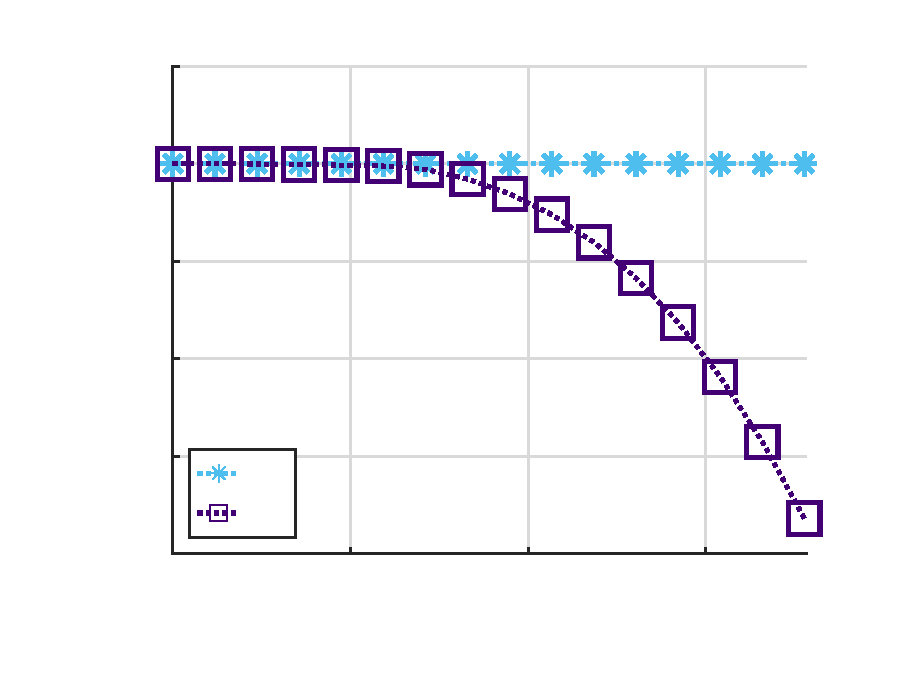
\includegraphics[scale=1]{BladeCantMomentXStatic-inc}
\end{picture}%
\begin{picture}(418,314)(0,0)
\fontsize{18}{0}\selectfont\put(74.9985,42.9569){\makebox(0,0)[t]{\textcolor[rgb]{0.15,0.15,0.15}{{$0$}}}}
\fontsize{18}{0}\selectfont\put(160.256,42.9569){\makebox(0,0)[t]{\textcolor[rgb]{0.15,0.15,0.15}{{$\pi/16$}}}}
\fontsize{18}{0}\selectfont\put(245.513,42.9569){\makebox(0,0)[t]{\textcolor[rgb]{0.15,0.15,0.15}{{$\pi/8$}}}}
\fontsize{18}{0}\selectfont\put(330.77,42.9569){\makebox(0,0)[t]{\textcolor[rgb]{0.15,0.15,0.15}{{$3\pi/16$}}}}
\fontsize{18}{0}\selectfont\put(66,56.4563){\makebox(0,0)[r]{\textcolor[rgb]{0.15,0.15,0.15}{{-2000}}}}
\fontsize{18}{0}\selectfont\put(66,103.254){\makebox(0,0)[r]{\textcolor[rgb]{0.15,0.15,0.15}{{-1500}}}}
\fontsize{18}{0}\selectfont\put(66,150.052){\makebox(0,0)[r]{\textcolor[rgb]{0.15,0.15,0.15}{{-1000}}}}
\fontsize{18}{0}\selectfont\put(66,196.851){\makebox(0,0)[r]{\textcolor[rgb]{0.15,0.15,0.15}{{-500}}}}
\fontsize{18}{0}\selectfont\put(66,243.649){\makebox(0,0)[r]{\textcolor[rgb]{0.15,0.15,0.15}{{0}}}}
\fontsize{18}{0}\selectfont\put(66,290.447){\makebox(0,0)[r]{\textcolor[rgb]{0.15,0.15,0.15}{{500}}}}
\fontsize{18}{0}\selectfont\put(226.972,18.9568){\makebox(0,0)[t]{\textcolor[rgb]{0.15,0.15,0.15}{{$\alpha$ [rad]}}}}
\fontsize{18}{0}\selectfont\put(19,173.452){\rotatebox{90}{\makebox(0,0)[b]{\textcolor[rgb]{0.15,0.15,0.15}{{$M_x$ node O [N.m]}}}}}
\fontsize{16}{0}\selectfont\put(110.983,95.1194){\makebox(0,0)[l]{\textcolor[rgb]{0,0,0}{{F1}}}}
\fontsize{16}{0}\selectfont\put(110.983,76.0077){\makebox(0,0)[l]{\textcolor[rgb]{0,0,0}{{F2}}}}
\end{picture}
}
	\caption{Example 3: Torsional moment $M_x(\alpha)$ at node O.}
	\label{fig:BladeCantMXStatic}
\end{figure}


\end{document}
